\subsection{Heimatforschung als Betätigungsfeld im Ruhestand}

Die Heimatkunde: Ein Hobby des
Pensionisten Högn? Nach Eintritt ins Rentenalter verfasste Högn drei
Geschichten mit heimatkundlichem Inhalt. Die lockere Abfolge ihrer
Entstehung vermittelt den Eindruck, dass sie eher unter einem Zustand
der Ablenkung, des Zeitvertreibs beziehungsweise der Zerstreuung
entstanden sind. Dies trifft bei Högn nur teilweise zu. Seine
schriftstellerische Tätigkeit kann auch mit der Vollendung einer von
der Gesellschaft an die Lehrer übertragenen Aufgabe umschrieben werden.

Eine Aktion der Regierung von Niederbayern zur Zeit der Weimarer
Republik mit dem Motto \zitat{„Pflege des
Heimatgedankens“}, \footnote{Dokument Nr. 133, Regierungsblatt zur
Pflege des Heimatgedankens, 12.11.1925} hatte das Ziel, durch
Heimatkunde, den Patriotismus und das Nationalbewusstsein der Bürger zu
stärken, um damit einen Beitrag zur Lösung der nationalen Probleme zu
leisten. Ein Rundschreiben vom 12.11.1925, das auch Högn vorlag, mit
dem Betreff \zitat{„Anlegung gemeindlicher Ortsgeschichten“}
macht die Intention dieser Aktion in wenigen Sätzen deutlich:
\zitat{„Die Voraussetzung für den Aufstieg unseres Volkes aus
dem jetzigen Tiefstande ist die Rückkehr zu deutscher Einfachheit,
Zucht und Sitte. Dazu muss der Sinn für die Heimaterde geweckt“} und
\zitat{„die Liebe zum Vaterlande entzündet [...] werden. Auf
diesen }\zitat{Grundlagen baut sich neben der körperlichen
und geistigen Ertüchtigung der Jugend die Zukunft des deutschen Reiches
auf.“} Vor allem \zitat{„die Herren Lehrer [...] sollten“
}daher\zitat{ „ohne weiteres Säumen und mit allem Nachdruck
[...] die Vorbereitung für die Herstellung der
Ortsgeschichten“} \footnote{Dokument Nr. 133, Regierungsblatt zur
Pflege des Heimatgedankens, 12.11.1925} aufnehmen. Dass die
angetragenen Vorhaben eine gewisse Verbindlichkeit hatten, zeigt schon
die Aufforderung, dass \zitat{„bis zum 1. April 1928
berichtet werden wolle, [...] in welchen Gemeinden die Vorarbeiten in
Angriff genommen worden sind (Anrede des Bearbeiters).“ }\footnote{
Dokument Nr. 133, Regierungsblatt zur Pflege des Heimatgedankens,
12.11.1925} Högn hat sich tatsächlich dieser Aufgabe angenommen, wie
die vielen heimatkundlichen Zeitungsartikel zeigen, die in der Zeit von
1926 bis 1928 erschienen sind. Doch es waren nur einzelne
heimatkundliche Beiträge, die entstanden sind. Die eigentlich
geforderte komplette Ortsgeschichte blieb aus. Stand der Vollendung
dieser Aufgabe die Zeitknappheit aufgrund des Schuldienstes in Wege, so
beseitigte seine Pensionierung dieses Hindernis zur umfassenden
Ortsgeschichte. \footnote{Dokument Nr. 133, Regierungsblatt zur Pflege
des Heimatgedankens, 12.11.1925} Bei der Geschichte von Zachenberg
etwa, gibt es ganz konkrete Anhaltspunkte, wonach die Initiative zur
Inangriffnahme der Arbeit nicht von Högn selbst aus ging, für den
Begriff Hobby ein notwendiges Merkmal, sondern eine an ihn
herangetragene Bitte den Grund für die Entstehung der Geschichte
lieferte.

\begin{flushleft}
\tablefirsthead{}
\tablehead{}
\tabletail{}
\tablelasttail{}
\begin{supertabular}{m{5.2310004cm}}

\begin{center}

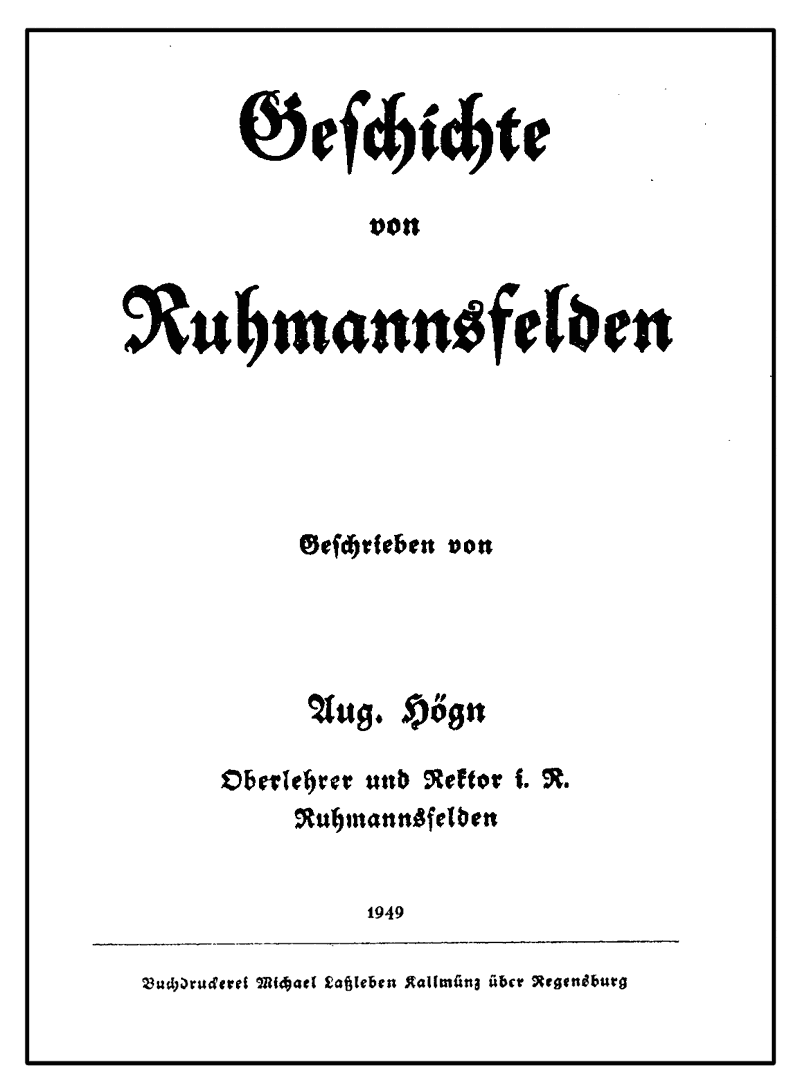
\includegraphics[width=4.995cm,height=6.833cm]{pictures/zulassungsarbeit-img040.png}

\end{center}
erste Seite der Geschichte von
Ruhmannsfelden\\
\end{supertabular}
\end{flushleft}

\begin{figure}
\img{}
\caption{}
\end{figure}

Gerade mal zwei Jahre nach Högns endgültiger Pensionierung,\footnote{
Dokument Nr. 48, Zeitungsartikel aus Viechtacher Bayerwald-Bote,
2.8.1958} erschien 1949 die „Geschichte von Ruhmannsfelden.“ Dem
rüstigen Rentner musste es eher leicht gefallen sein, Material für
seine Arbeit zu finden, konnte er doch auf eine rege Forschertätigkeit
vergangener Jahrzehnte zurückblicken und brauchte die vielen bereits
existierenden Einzelbeiträge zur Heimatgeschichte nur noch in einem
Werk zusammenfassen. Die geschichtliche Entwicklung zwei wichtiger
Institutionen am Ort hatte Högn lange vor dem 2. Weltkrieg bearbeitet:
Die Entwicklung der Ruhmannsfeldener Schule war in einer Beilage zum
Deggendorfer Donauboten 1927 erschienen und anlässlich der 100-jährigen
Einweihungsfeier der Ruhmannsfeldener Pfarrkirche wurde 1928 bis 1929
in mehreren Teilen die Geschichte der Pfarrkirche St. Laurentius im
Viechtacher Tagblatt abgedruckt. Information über die Entstehung des
Namens „Ruhmannsfelden“ oder den Zeitpunkt der Marktrechtsverleihung
beinhalteten zwei Zeitungsartikel aus dem Jahre 1926 und fanden an
exponierter Stelle Eingang in die „Geschichte von Ruhmannsfelden“. Es
war August Högn, der sich zur Frage des Namensursprungs von
„Ruhmannsfelden“ schon 1922 an den Straubinger Historiker Dr. Joseph
Keim wandte \footnote{Dokument Nr. 20, Brief von Dr. Keim an August
Högn, 30.8.1922} und die noch heute gültige Erklärung gab, wonach
Ruhmannsfelden nach dem Rodungsarbeiter „Rumar“ benannt wurde. Davor
wurde der Name „Ruhmannsfelden“ etwas trivial mit „Ruht der Mann in
Felde“ erklärt. \footnote{Interview Nr. 9, Dr. Doraliesa Wiegmann,
19.1.2003, Absatz 4} Ebenso versuchte Högn sowohl in dem erwähnten
Artikel als auch in der „Geschichte von Ruhmannsfelden“ dem Mythos,
dass einst ein Schloss am Leitenberg bestand, entgegenzuwirken. Trotz
aller realisierbaren Recherchearbeiten ist es unverkennbar, dass Högn
besonders zur frühen Geschichte Ruhmannsfeldens auf sehr wenige
Informationen zurückgreifen konnte. Das einleitende Kapitel der
Geschichte von Ruhmannsfelden „Wie hat es vor seiner Entstehung
ausgesehen?“ ähnelt in seinem Aufbau mehr einem Roman als dem Beginn
einer historischen Abhandlung und entbehrt sicherlich aller
wissenschaftlichen Beweise. Wegen fehlender Dokumente musste von Namen
wie etwa „Ruhmannsfelden“ oder „Laurentius-Kirche“ auf die mögliche
geschichtliche Entwicklung geschlossen werden. Manchmal schlussfolgerte
Högn aus diesen Anhaltspunkten etwas zuviel. Es stimmt sicher, dass
alle dem hl. Laurentius geweihten Kirchen außerhalb der Ortschaften
standen, aber dass die „Laurentius“-Kirche in Ruhmannsfelden zuerst aus
Holz war, unter den Aldersbachern dann aus Stein und dass dann auch
öfter Gottesdienste stattfanden, wie in der Geschichte von
Ruhmannsfelden steht, ist wohl rein Spekulation. \footnote{Högn,
Ruhmannsfelden, Seite 10} Als Lückenfüller dürften die Kapitel über die
Namen der Ruhmannsfeldener Fluren und Gassen und eine Auflistung der
Höhenlagen mit Barometerstand der umliegenden Berge und Ortschaften
gedient haben.

Der Entstehungsgrund der „Geschichte und Chronik der freiwilligen
Feuerwehr Ruhmannsfelden“ ist eng mit dem Ende von Högns
Schriftführertätigkeit bei der Feuerwehr verbunden. Am Stefani-Tag 1950
wurde Johann Freisinger zum Schriftführer der Feuerwehr Ruhmannsfelden
gewählt und löste somit August Högn nach 40-jähriger Dienstzeit ab. Die
\zitat{„in dankbarer Erinnerung“}  \footnote{Högn,
Ruhmannsfelden, Titelblatt} der Feuerwehr gewidmete Geschichte hat Högn
geschrieben, um seine Tätigkeit als Schriftführer abzurunden und sein
in 40 Jahren gesammeltes Wissen in diese Arbeit einfließen zu lassen.
Ein passender Übergabetermin der Chronik an die Feuerwehr wäre der zur
Verabschiedung von Högn eigens veranstaltete Ehrenabend am 11. März
1951 gewesen, doch die Chronik wurde der letzten Eintragung zufolge
erst nach dem 1. April 1951 fertig geschrieben. Aber die Arbeit war zum
Ehrenabend der Feuerwehr schon versprochen und fand deswegen lobende
Erwähnung in der Abschiedesrede des Feuerwehrkommandanten.\footnote{
Dokument Nr. 110, Abschiedsrede des Feuerwehrkommandanten Johann
Linsmeier, 3.11.1951} Die fertige Chronik überreichte Högn persönlich
dann kurze Zeit später seinem Schriftführer-Nachfolger.\footnote{
Interview Nr. 14, Johann Freisinger, 29.12.2003, Absatz 16} Die
Abhandlung ist nach Jahrgängen gegliedert und lässt daher oft
Einzelfakten unverbunden nebeneinander stehen, was das Verständnis beim
Lesen erschwert. Sie ist deshalb wohl eher als eine Stoffsammlung zur
weiteren Bearbeitung anzusehen, als ein unterhaltsamer Lesestoff für
die breite Ruhmannsfeldener Bevölkerung und war sicher nie für den
Druck bestimmt. Lediglich die länger ausformulierte Gründung der
Feuerwehr und der Bericht samt Querverweisen über den sich über
längeren Zeitraum erstreckende und deshalb in mehreren Jahren
auftauchende Streit der Gemeinden Ruhmannsfelden und Zachenberg um eine
gemeinsam angeschaffte Feuerwehrspritze bleiben dem Leser in Erinnerung
und gehen nicht in der Flut von Einzelinformationen unter.

\begin{center}
\begin{minipage}{10.007cm}
\begin{flushleft}
\tablefirsthead{}
\tablehead{}
\tabletail{}
\tablelasttail{}
\begin{supertabular}{m{5.0280004cm}m{4.578cm}}

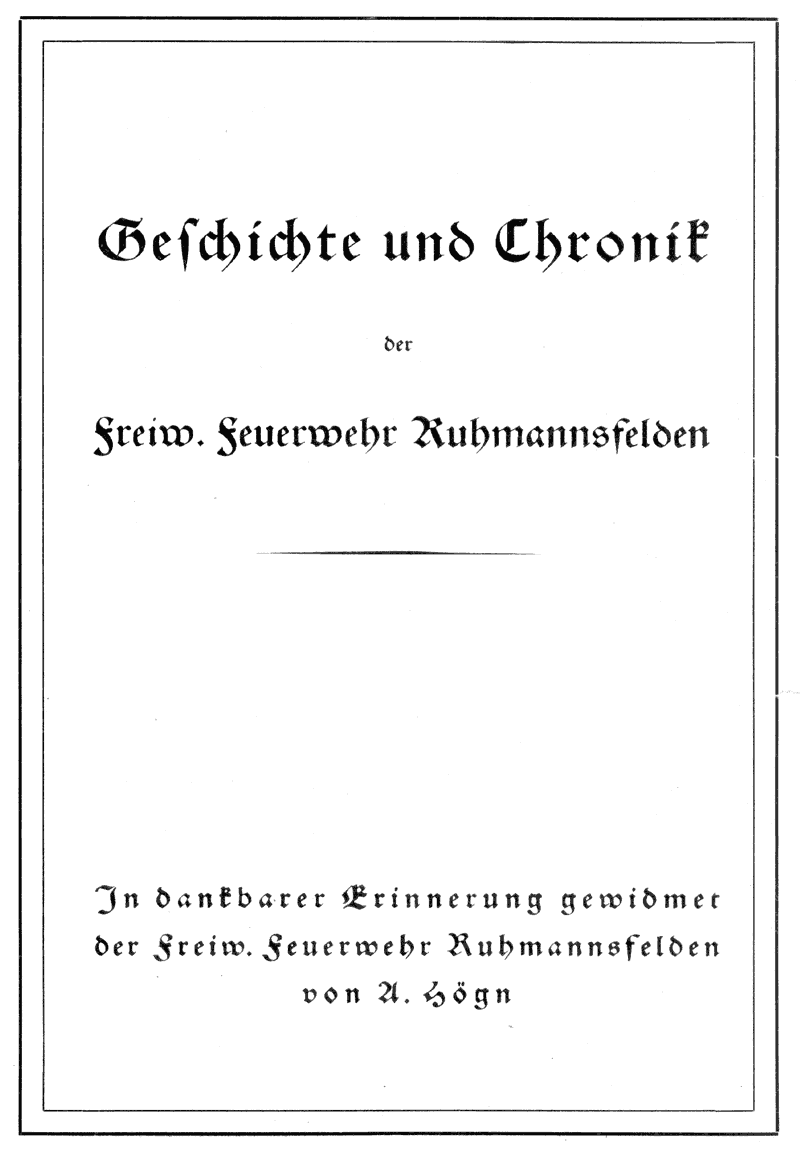
\includegraphics[width=4.847cm,height=6.997cm]{pictures/zulassungsarbeit-img041.png}

Deckblatt des Manuskripts der
„Geschichte und Chronik der Freiw. Feuerwehr Ruhmannsfelden“ &

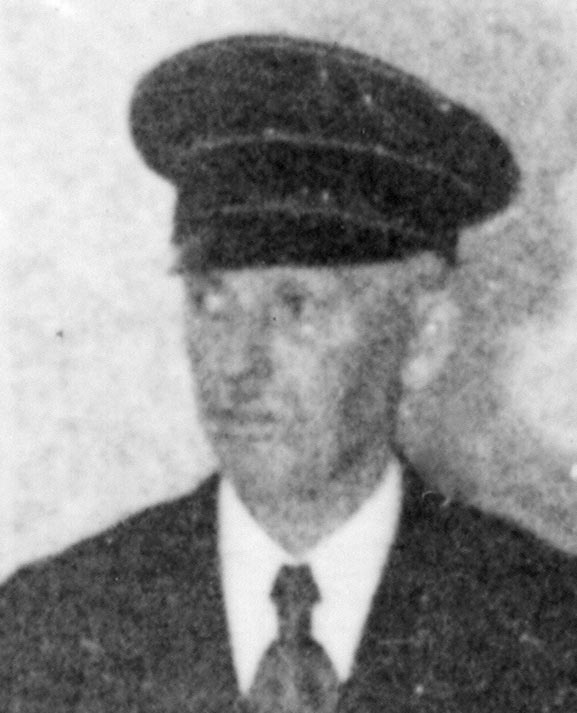
\includegraphics[width=4.396cm,height=6.997cm]{pictures/zulassungsarbeit-img042.jpg}

August Högn bei der Mitglieder-Ehrung
der Feuerwehr 1950\\
\end{supertabular}
\end{flushleft}
\end{minipage}
\end{center}

\begin{figure}
\img{}
\caption{}
\end{figure}

Ein auswärtiger, nicht in der Gemeinde Zachenberg ansässiger Bürger
lieferte die Initiative zur Entstehung von Högns „Heimat-Geschichte der
Gemeinde Zachenberg.“ Der Finanzzollrat Anton Trellinger – er war am
Landshuter Hauptstaatsarchiv als Archivpfleger angestellt – fertigte
einen 63-seitigen Akten-Auszug \footnote{Dokument Nr. 31, Brief von
August Högn an Klosterbibliothekar des Klosters Niederalteich,
26.3.1952, Dokument Nr. 33, Brief von August Högn an das Pfarramt
Grafenau, 26.3.1952} über die Gemeinde Zachenberg an. Da Trellinger die
Gemeinde Zachenberg nur flüchtig kannte und gesundheitlich sehr
angeschlagen war, \footnote{Dokument Nr. 28, Brief von Finanzzollrat
Anton Trellinger an August Högn, 25.2.1952} – er erlitt im Frühjahr
1952 einen Schlaganfall \footnote{Dokument Nr. 35, Brief von Expositus
Georg Hofmann, Schönau an August Högn, 23.10.1952} – bat er seinem
Brief die Gemeinde Zachenberg um einen ortskundigen Fachmann, der seine
Arbeit ergänzen und fortführen könnte. Den Sachbearbeitern bei der
Gemeinde dürfte es nicht schwer gefallen sein, Trellinger die
geforderte Person zu nennen: August Högn. Lange bevor Anton Trellinger
der Gemeinde Zachenberg seine Arbeit übersandte, nämlich am 25.2.1952,
und am selben Tag Högn persönlich anschrieb, \footnote{Dokument Nr. 28,
Brief von Finanzzollrat Anton Trellinger an August Högn, 25.2.1952}
hatte August Högn schon mit der Recherche begonnen und den Mettener
Benediktiner-Pater Wilhelm Fink von der beabsichtigen Geschichte von
Zachenberg in Kenntnis gesetzt und um wissenschaftliche Betreuung
gebeten. \footnote{Dokument Nr. 29, Brief von Pater Wilhelm Fink an
August Högn, 28.1.1952}

\begin{center}
\begin{minipage}{5.378cm}
\begin{flushleft}
\tablefirsthead{}
\tablehead{}
\tabletail{}
\tablelasttail{}
\begin{supertabular}{m{5.178cm}}

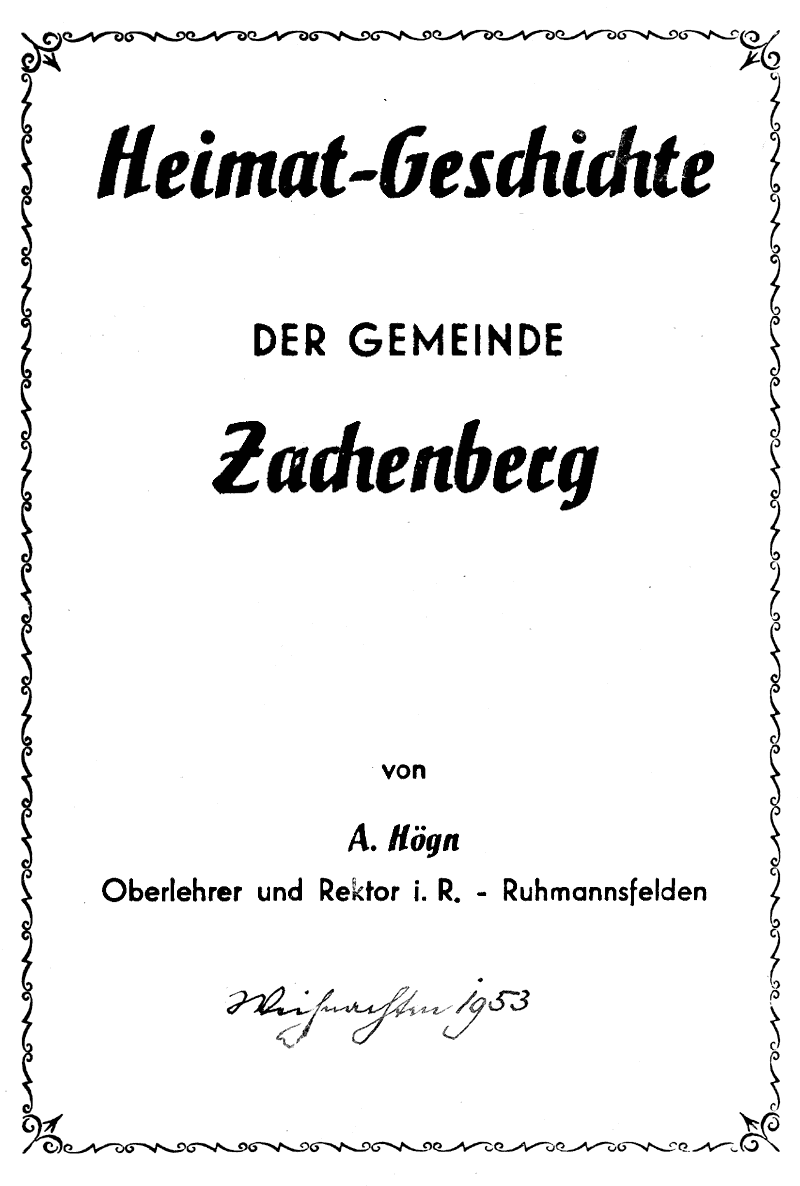
\includegraphics[width=4.995cm,height=7.405cm]{pictures/zulassungsarbeit-img043.png}

Deckblatt des Manuskripts der
„Heimat-Geschichte der Gemeinde Zachenberg“\\
\end{supertabular}
\end{flushleft}
\end{minipage}
\end{center}
Trellinger lieferte mit seinen Archivauszügen nicht nur einen wichtigen
Grundstock für Högns „Heimat-Geschichte der Gemeinde Zachenberg“,
sondern er gab ihm auch einige Tipps und Literaturhinweise.\footnote{
Dokument Nr. 28, Brief von Finanzzollrat Anton Trellinger an August
Högn, 25.2.1952} Nach fast 2-jähriger Arbeitszeit wurde die „Geschichte
von Zachenberg“ an Weihnachten 1953 fertig gestellt \footnote{Högn,
Zachenberg, Deckblatt} und an Wilhelm Fink zum Korrekturlesen
übersandt. Fink hatte besonders zum 1. Teil der Abhandlung einige
Änderungsvorschläge anzubieten. Es ist deshalb nicht verwunderlich,
dass sich die ersten Teile der „Geschichte von Ruhmannsfelden“ und der
„Geschichte von Zachenberg“ im Aufbau und in der Darstellung ziemlich
stark unterscheiden, obwohl beide Teile die geschichtliche Entwicklung
von den Anfängen der beiden benachbarten und sich unter den gleichen
Herrschaftsverhältnissen entwickelnden Gemeinden zum Thema haben. Fink
hat offensichtlich die „Geschichte von Ruhmannsfelden“ nicht Korrektur
gelesen. Im von Fink als druckreif befunden 2. Teil der Geschichte von
Zachenberg geht Högn auf die 15 Dörfer, 13 Weiler und 10 Einöde, also
auf die insgesamt 38 Ortschaften der Gemeinde Zachenberg im Einzelnen
ein.

Die Kapitel über die einzelnen Ortschaften ähneln mehr genealogischen
Studien als historischen Abhandlungen. Manchmal lassen sich aus diesen
Kapiteln Stammbäume einzelner Bauernfamilien über Jahrhunderte hinweg
ablesen. Meistens jedoch konnten die Angaben aus den sehr alten
Aktenauszügen Trellingers nicht mit den neueren Informationen aus dem
Gemeindearchiv oder von den befragten Bewohnern der jeweiligen
Ortschaft bruchlos aneinander gereiht werden. Die sehr schematische
Beschreibung der kleinsten Ortschaften selbst – sie beginnt immer mit
der Herkunfts-Erklärung des Ortsnamens und endet nach Vorstellung der
einzelnen Bauernfamilien mit Angabe der damals aktuellen Einwohner- und
Häuserzahl – wird durch Sagen und Erzählungen aufgelockert, die Högn
von älteren Bewohnern der einzelnen Orte erzählt bekam und sie in Form
von Nacherzählungen wiedergibt. Viele der von Wilhelm Fink
vorgeschlagenen Ergänzungen zum dritten, allgemeinen Teil – hier geht
es in erster Linie um die damalige aktuelle Organisation der Gemeinde –
hat Högn nicht angenommen, weil beiden Gemeinden, Zachenberg und
Ruhmannsfelden, doch sehr ähnliche Strukturen aufwiesen und er bereits
Einiges in der Geschichte von Ruhmannsfelden erwähnt hatte, wie zum
Beispiel die aus der Pfarrei hervorgegangenen Priester, die Lehrer oder
die Polizei. Deshalb erörtert er hier hauptsächlich die aktuellen
wirtschaftlichen und infrastrukturellen Aspekte der Gemeinde
Zachenberg. \footnote{Dokument Nr. 38, Brief von Pater Wilhelm Fink,
Metten an August Högn, 23.2.1954}

Als er die korrigierte Fassung der Geschichte kurz vor Ostern 1954 der
Gemeinde Zachenberg übergab, rechnete er sicher mit einer schnellen
Drucklegung seiner Arbeit, ähnlich wie bei der Geschichte von
Ruhmannsfelden, sonst hätte er sich nicht schon von der Druckerei
Michael Laßleben in Kallmünz ein Angebot geben lassen und sich sogar
schon einen Werbetext für ein Inserat oder ein Plakat
überlegt. \footnote{Dokument Nr. 39, Brief von August Högn an
Bürgermeister Ludwig Bielmeier, Zachenberg, 31.3.1954}

\begin{center}
\begin{minipage}{5.812cm}
\begin{center}
\tablefirsthead{}
\tablehead{}
\tabletail{}
\tablelasttail{}
\begin{supertabular}{m{5.612cm}}

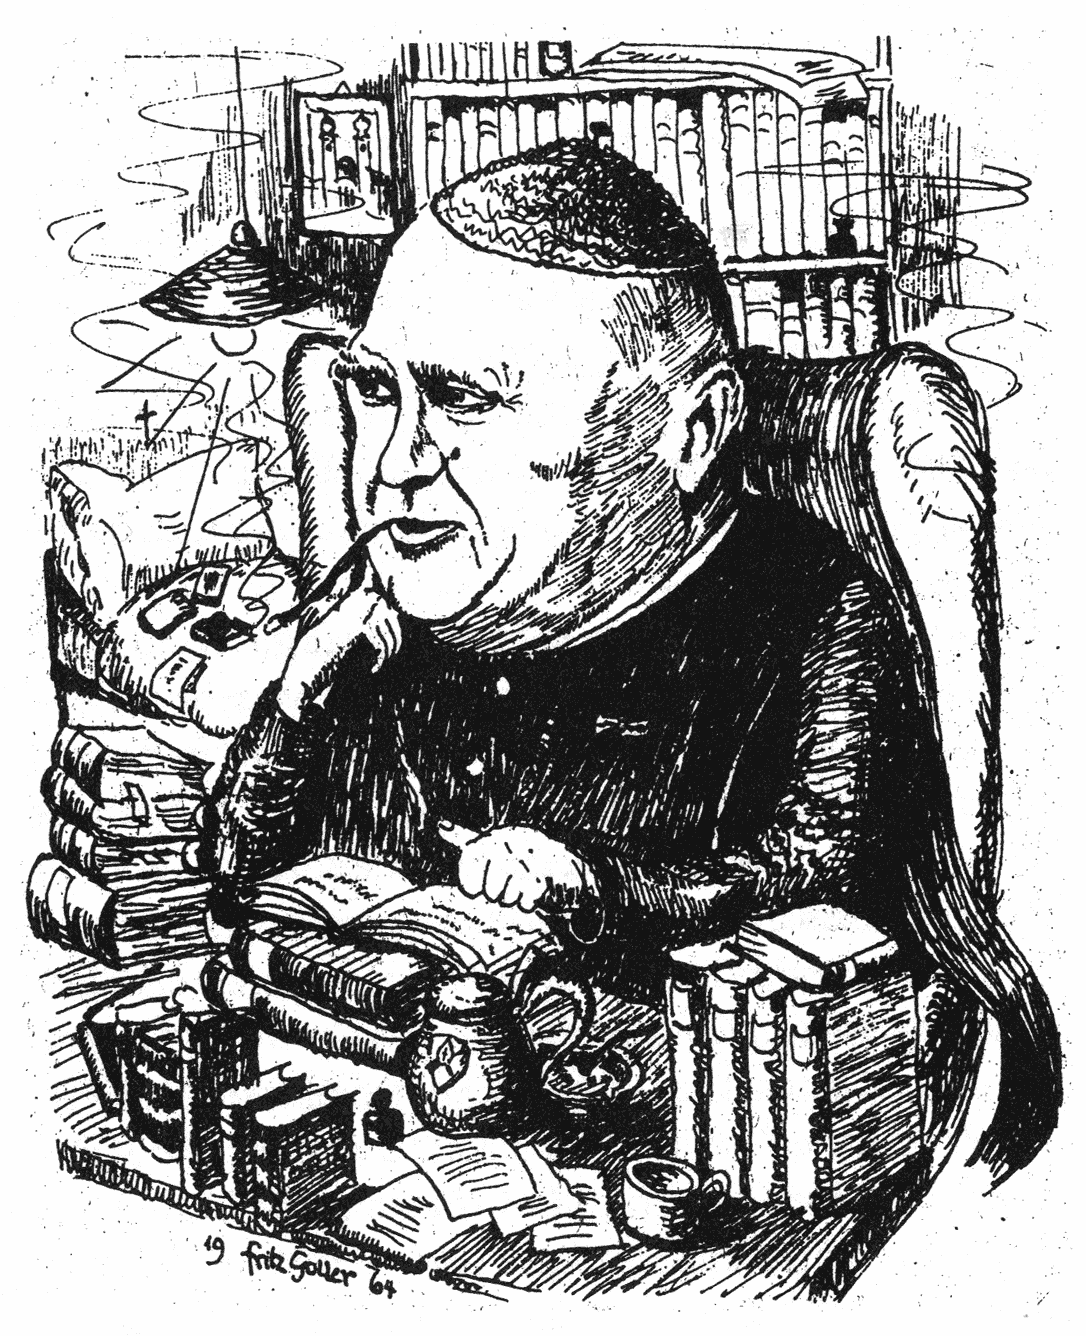
\includegraphics[width=5.429cm,height=6.68cm]{pictures/zulassungsarbeit-img044.png}

Wilhelm Fink in einer Karikatur von
Fritz Goller\\
\end{supertabular}
\end{center}
\end{minipage}
\end{center}

\begin{figure}
\img{}
\caption{}
\end{figure}

Erst am 7. Mai 1956 versicherte der Zachenberger Bürgermeister Bielmeier
August Högn, auf seine Anfrage hin, dass der Gemeinderat über die
Veröffentlichung der „Geschichte von Zachenberg“ in der nächsten
Sitzung beraten würde. \footnote{Dokument Nr. 40, Brief von
Bürgermeister Ludwig Bielmeier, Zachenberg an August Högn, 7.5.1956}
Die Gemeindevorsteher hatten wohl von Anfang an kein Interesse an einer
Drucklegung. \footnote{Interview Nr. 14, Johann Freisinger, 29.12.2003,
Absatz 13 – 14} Kein einziges Wort ist über den Druck des Buchs im
Protokoll der Gemeinderatssitzung vom 17.5.1956 zu finden. Stattdessen
wurde beschlossen, Högn zum Ehrenbürger der Gemeinde Zachenberg zu
ernennen und ihm als \zitat{„Entschädigung“ }für seine
Bemühungen ein \zitat{„Geldgeschenk im Ermessen des 1.
Bürgermeisters“} \footnote{Dokument Nr. 96,
Sitzungsprotokoll des Gemeinderats Zachenberg, 17.5.1956} zukommen zu
lassen. Trotz aller dieser Ehren dürfte die immer noch nicht
eingeleitete Vervielfältigung der „Geschichte von Zachenberg“ eine
Enttäuschung für Högn gewesen sein. Noch an seinem 80. Geburtstag, also
über 4 Jahre nach der Fertigstellung des Werks, machte er sich Hoffnung
auf eine baldige Drucklegung des Werks, \footnote{Dokument Nr. 48,
Zeitungsartikel aus Viechtacher Bayerwald-Bote, 2.8.1958} die bis zum
heutigen Tag auf sich warten lässt.

\begin{flushleft}
\tablefirsthead{}
\tablehead{}
\tabletail{}
\tablelasttail{}
\begin{supertabular}{m{3.7879999cm}}

\begin{center}

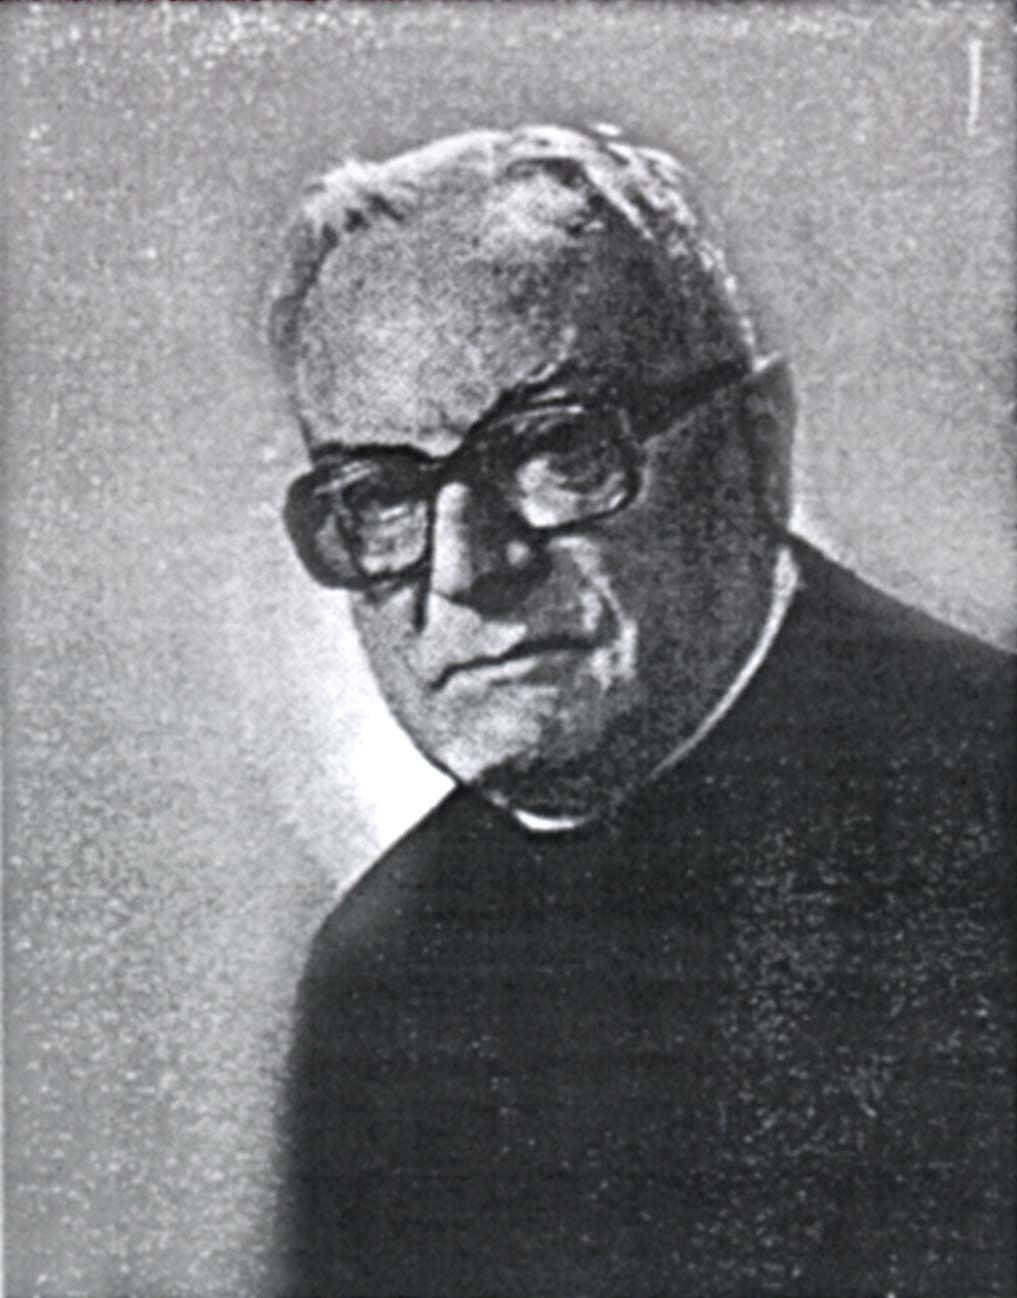
\includegraphics[width=3.605cm,height=4.6cm]{pictures/zulassungsarbeit-img045.jpg}

\end{center}
Ferdinand Haberl\\
\end{supertabular}
\end{flushleft}

\begin{figure}
\img{}
\caption{}
\end{figure}

August Högn war nicht nur auf heimatkundlichem Gebiet schriftstellerisch
tätig. Es gibt Anzeichen dafür, dass er sich auch mit musikhistorischen
Themen beschäftigt haben könnte. Ein Briefwechsel aus dem Jahr 1947 mit
Ferdinand Haberl, Direktor der Kirchenmusikschule in Regensburg, in dem
es um die Entstehung und Herkunft des Weihnachtsliedes „Stille Nacht“
geht, unterstreicht diese Annahme. \footnote{Dokument Nr. 65, Brief von
August Högn an Dr. Haberl, Regensburg, Mrz. 1947; Dokument Nr. 61,
Brief von F. Mitterwallner, Deggendorf an August Högn, 25.2.1947}
